\documentclass[11pt,ngerman,a4paper]{article}
%Gummi|061|=)
\usepackage{amsmath}
\usepackage{a4wide}
\usepackage{url}
\usepackage{amsthm}
\usepackage{amsbsy}
\usepackage{amssymb}
\usepackage[utf8]{inputenc}
\usepackage{rotating} 
\usepackage{here}
\usepackage{graphicx}
\usepackage{paralist}
\usepackage{selinput}
\usepackage[separate-uncertainty=true]{siunitx}
\usepackage{booktabs}
\sisetup{}
\SelectInputMappings{%
adieresis={ä},
germandbls={ß},
}
\title{\textbf{Versuch V504: Thermische Elektronenemission}}
\author{Martin Bieker\\
		Julian Surmann\\
		\\
		Durchgef\"{u}hrt am 17.06.2014\\
		TU Dortmund}
\date{}
\usepackage{graphicx}
\begin{document}
\renewcommand\tablename{Tabelle}
\renewcommand\figurename{Abbildung}
\maketitle
\thispagestyle{empty}
\newpage
\clearpage
\setcounter{page}{1}


\section{Einleitung}
In diesem Versuch wird die sogenannte Thermische Elektronenemission untersucht, dabei handelt es sich um die Auslösung von Elektronen aus einer Metalloberfläche mit Hilfe von thermischer Energie. Die Temperaturabhängigkeit dieses Vorganges ist von besonderem Interesse.
\section{Theorie}
\section{Auswertung}
\subsection{Bestimmung des Sättigungsstroms}
Zur Bestimmung des temperaturabhängigen Sättigungsstroms der Diode wurde der Strom in Abhängigkeit vom der Spannung zwischen Anode und Kathode gemessen. Diese Daten befinden sich in Tabelle \ref{tab_a}. In Abbildung \ref{abb_a} werden die ermittelten Kennlinien graphisch dargestellt. 
\begin{figure}[htp]
\centering
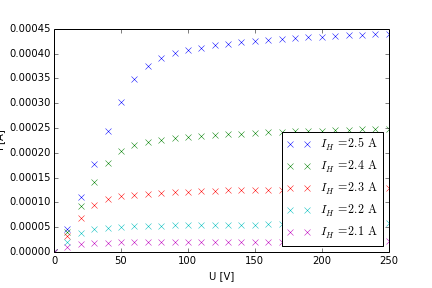
\includegraphics[scale=0.8]{plot_a.png}
\caption{Kennlinie der Hochvakuumdiode in Abhängigkeit von der Temperatur.}
\label{abb_a}
\end{figure}

\noindent
Es ist erkennbar, dass der Strom innerhalb des untersuchten Spannungsbereichs das jeweilige temperaturabhängige Sättigungsniveau erreicht. Somit entspricht der Sättigungsstrom näherungsweise dem höchsten gemessenen Wert von $I$ der jeweiligen Messreihe. Daher gilt:
\begin{itemize}
\item $I_1 = \SI{440}{\micro\ampere}$
\item $I_2 = \SI{248}{\micro\ampere}$
\item $I_3 = \SI{129}{\micro\ampere}$
\item $I_4 = \SI{58}{\micro\ampere}$
\item $I_5 = \SI{22}{\micro\ampere}$
\end{itemize}

\subsection{Verifizierung Langmuir-Schottkyschen Gesetztes}
In diesem Versuchsteil wird das Raumladungsgebiet der Kennlinie genauer untersucht.
Hier soll der Exponent $q$ der Strom-Spannungsbeziehung 
\[
I = k\cdot x^q
\]
bestimmt werden. Dazu sind in Abbildung \ref{plot_b} sind die Messpunkte für die maximale Heizleistung ($I_H = \SI{2.5}{\ampere}$) doppelt logarithmisch aufgetragen. In dieser Darstellung ist der lineare Zusammenhang
\[
\ln\left(\frac{I}{\si{\ampere}}\right) = q\cdot \ln\left(\frac{U}{\si{\volt}}\right)+ \ln\left(\frac{k}{\si{\ampere\per\volt}}\right)
\]
erkennbar. Durch eine lineare Ausgleichsrechnung ergibt sich:
\begin{itemize}
\item $q = \num{1.1317+-0.0011}$
\item $\ln\left(\frac{k}{\si{\ampere\per\volt}}\right) = \num{-12.531+-0.013}$ 
\end{itemize}
Die durch diese Werte bestimmte Ausgleichsgerade ist ebenfalls in Abbildung \ref{plot_b} dargestellt.
Die Abweichung von $q$ zum Langmuir-Schottkyschen Gesetz mit 
\[
q_{theo} = \frac32
\]
beträgt:
\[
\Delta q = \frac{|q_{theo}-q|}{q_{theo}} = \SI{24.55}{\percent}\rm.
\]
\subsection{Untersuchung des Anlaufstromgebiets}
Tabelle \ref{tab_c} enthält den gemessenen Diodenstrom $I$ in Abhängigkeit von der angelegten Gegenspannung $U$. Diese Messwerte sind in Abbildung \ref{plot_c_lin} graphisch dargestellt. Es zeigt sich der erwartete exponentielle Zusammenhang
\[
I = C\cdot \exp\left(\frac{e_0 U}{k_b T}\right)\rm.
\]
Daher werden die Messwerte in Abbildung \ref{plot_c_log} halb-logarithmisch aufgetragen. Es ergibt sich der folgende lineare Zusammenhang:
\[
\ln{\left(\frac{I}{\si{\ampere}}\right)} = \frac{e_0}{k_b T }\cdot U + \ln(C)\rm = m \cdot U + b.
\]
Durch eine lineare Regression wird die Steigung $m$ der Geraden bestimmt. Es ergibt sich:
\[
m = \num{-4.198+-0.004} = \frac{e_0}{k_b T} \Leftrightarrow T = \SI{2764.2+-2.7
}{\kelvin}
\] 
\subsection{Bestimmung der Temperatur der Kathode}

Aus einer Leistungsbilanz kann die Temperatur der Kathode bestimmt werden. Denn es gilt:
\[
N_{el} = N_{WL} + N_{Str.}\rm.
\]
Die Elektrische Heizleistung kann aus Heizstrom und Heizspannung berechnet werden. Die Strahlungsleistung kann durch das Stefan-Boltzmannsche Gesetz
\[
N_{Str.} = A \eta\sigma T^4
\]
ausgedrückt werden. Da die Fläche der Kathode 
\[
A = \SI{0,32}{\centi\meter\squared}
\]
die Stefan-Boltzmannsche Konstante 
\[
\sigma = \SI{}{\watt\per(\centi\meter\squared\kelvin^4)}
\]
und der Absorptionsgrad
\[
\eta = \num{0,27}
\]
bekannt sind und der Energieverlust durch Wärmeleitung durch
\[
N_{WL} = \SI{1}{\watt}
\]
abgeschätzt werden kann, gilt für die Temperatur:
\[
T = \sqrt[4]{\frac{U_H I_H - \SI{1}{\watt}}{A\eta\sigma}}\rm.
\]
Die Ergebnisse dieser Berechnungen befinden sich in Tabelle \ref{tab_d}.

\subsection{Berechnung der Austrittsarbeit des Kathodenmaterials}
Aus den in den vorherigen Teilen der Auswertung bestimmten Werten für den Sättigungsstrom $I_S$ der dazugeörigen Kathodentemperatur $T$ kann mit Hilfe der Richardson-Gleichung (Formel \ref{}) die Austrittsarbeit des Kathodenmaterials bestimmt werden. Es gilt:
\[
W_A = -\log\left( \frac{I_S h^3}{e_0 m_0 k_b^2 T^2}\right)\cdot k_b T
\]
Die mit dieser Formel berechneten Werte befinden sich in Tabelle \ref{tab_e}. Es ergibt sich für den Mittelwert mit statistischen Fehler:
\[
 W_A = \SI{6.32+-0.05}{\eV}\rm.
\]
Die Kathode der in diesem Versuch verwendeten Diode besteht aus Wolfram. Der Literaturwert[2] für die Austrittsarbeit beträgt
\[
W_A \approx \SI{4,6}{\eV}
\]
Damit berechnet sich die Abweichung des experimentell bestimmten Wertes vom Literatur-wert zu
\[
\Delta W_A = \frac{|W_A-\overline{W_A}|}{W_A} = \SI{38,79}{\percent} 
\]

\section{Diskussion}

\section{Quellen}
\begin{enumerate}[{[}1{]}]
\item Entnommen der Praktikumsanleitung \textit{} der TU Dortmund. \\
Download am 01.06.14 unter:\\
 \url{http://129.217.224.2/HOMEPAGE/PHYSIKER/BACHELOR/AP/SKRIPT/V703.pdf}
\end{enumerate}

\section{Anhang}
\begin{itemize}
\item Tabellen
\item Auszug aus dem Messheft
\end{itemize}
\end{document}
